\chapter{REVISÃO DE LITERATURA}\label{chap:fundamentacaoTeorica}

Para o presente trabalho, em decorrência dos instrumentos e sensores escolhidos, devemos colher na literatura as equações e formalismos que descrevem o movimento e a orientação dos corpos no espaço, bem como as relações com as forças envolvidas. Além da literatura básica sobre mecânica v.~\cite{Goldstein1980}, robótica v.~\cite{Craig2014} e controle v.~\cite{Ogata2010}, os temas são mais bem explorados na literatura sobre controle de aeronaves e mísseis v.~\cite{Henderson1997}, \cite{Stevens2016}, \cite{Blakelock1991} ou sobre navegação inercial v.~\cite{Stovall1997}, \cite{Weston2004}, \cite{Wang2021} e~\cite{Haoran2019}

No particular, empregaremos em grande parte as convenções e equações utilizadas em~\cite{Stevens2016}, que acreditamos dar um tratamento mais direto e acessível a esses temas.

\section{Notação e convenções}

Neste trabalho utilizamos um modelo de mundo tridimensional e mecânica clássica.  Nosso espaço é estruturado por três eixos ortogonais \(x\), \(y\), \(z\) (\(1, 2, 3\)) onde uma posição é dada por um vetor tridimensional. Descreveremos a atitude e o movimento de um corpo rígido sobre a superfície oblata e girante da Terra. Não obstante, serão empregadas aproximações sobre uma pequena área para uma terra plana, estacionária e constante, que basta\footnotemark{} para os nossos propósitos.

\begin{align*}
    \mathbf{p}_{A/B} &\equiv
    \text{ vetor posição do ponto A em relação ao ponto B} \\
    \mathbf{v}_{A/i} &\equiv
    \text{ vetor velocidade do ponto \(A\) no quadro \(F_{i}\)} \\
    ^{b}\mathbf{\dot{v}}_{A/i} &\equiv
    \text{ vetor derivada de \(\mathbf{v}_{A/i}\) tomada no sistema \( F_{b}\)} \\
    \mathbf{v}^{c}_{A/i} &\equiv \left( \mathbf{v}_{A/i} \right)^{c} \equiv
    \text{ conjunto dos componentes de \(\mathbf{v}_{A/i}\) no sistema de coordenadas \(c\)} \\
\end{align*}

Componentes de vetores terão índices para indicar o sistema de coordenadas ou serão denotados pelo símbolo de vetor com índices \(x\), \(y\), e \(z\) para indicar as coordenadas, exceto quando indicado pelo símbolo transposto, e todos vetores são do tipo vetor coluna. Por exemplo:
\begin{align*}
    &\mathbf{p}^{b}_{A/B} = \begin{bmatrix}x_{b} \\ y_{b} \\ z_{b}\end{bmatrix}&
    \text{ ou }&
    &\mathbf{v}^{b}_{A/i} = \begin{bmatrix} v_{x} \\ v_{y} \\ v_{z} \end{bmatrix} = \begin{bmatrix} v_{x} & v_{y} & v_{z} \end{bmatrix}^{T}
\end{align*}

\footnotetext{A título de advertência, o assunto não é simples, com diversos formalismos possíveis, um campo fértil para confusão. Por exemplo, a atitude de um corpo pode ser descrita em três dimensões com ângulos de Euler ao menos em doze sequências de rotações anti-horárias distintas, não intercambiáveis, ou ainda pode ser descrita em quatro dimensões com o uso do quaternion, conforme observamos em~\cite{Henderson1997}. Além disso, é importante separar a orientação relativa do nosso espaço tridimensional em abstrato, do eixo de referência em relação ao nosso espaço abstrato, e do sistema móvel que pretendemos descrever em relação ao sistema de referência. No presente trabalho adotaremos um único formalismo que atende aos nossos propósitos limitados, e remetemos o leitor às fontes para aprofundamento do assunto.}

\section{Descrevendo a atitude de um corpo}

Descrevemos a atitude de um robô em ângulos de Euler na sequência \(z\), \(y\), \(x\) (3, 2, 1) que leva de um sistema de referência fixo na Terra até um sistema fixo no corpo do robô. Escolhemos o sistema (\(ned\)) - ``North-East-Down'' (Norte, Leste, Abaixo) com o eixo \(x\) apontando par o Norte, o eixo \(z\) Abaixo, o eixo \(y\) completando o sistema de coordenadas, e o sistema (\(frd\)) - ``Front-Right-Down'' (Avante, Direita, Abaixo) fixo no robô são, com eixos, respectivamente, (\(x\),\(y\),\(z\)), sendo o Avante alinhado à \emph{linha de referência longitudinal} do robô, com os eixos  ``Avante'' e ``Abaixo'' situados no plano de simetria, e o eixo Direito completando o sistema. Adotamos, ainda a convenção de rotações anti-horárias (regra da mão direita).

Desse a modo, a sequência de rotações que leva do sistema de referência \(ned\) para o sistema \(frd\) no corpo é dada por:
\begin{enumerate}
    \item Rotação anti-horária sobre eixo \(z\), ou \(\psi\) positivo (\textit{``compass heading''})
    \item Rotação anti-horária sobre novo eixo \(y'\), ou \(\theta\) positivo (\textit{pitch})
    \item Rotação anti-horária sobre novo eixo \(x''\), ou \(\phi\) positivo (\textit{roll})
\end{enumerate}

Esta sequência de rotações é normalmente denominada \emph{``yaw, pitch, roll''} (guinada, arfada e rolagem), partindo do sistema de referência.

Podemos escrever as matriz de rotação abreviando co-seno por \(c\) e seno por \(s\). Esta matriz representa uma transformação padrão que será utilizada ao longo do texto:

\begin{align*}
    C_{f\!r\!d\!/\!n\!e\!d} =
    \begin{bmatrix}
        1               &  0            &  0             \\
        0               &  \cos{\phi}   &  \sin{\phi}    \\
        0               & -\sin{\phi}   &  \cos{\phi}
    \end{bmatrix}
    \begin{bmatrix}
        \cos{ \theta}   &  0            & -\sin{\theta} \\
        0               &  1            &  0            \\
        \sin{ \theta}   &  0            &  \cos{\theta}
    \end{bmatrix}
    \begin{bmatrix}
        \cos{\psi}      &  \sin{\psi}   &  0             \\
       -\sin{\psi}      &  \cos{\psi}   &  0             \\
        0               &  0            &  1
    \end{bmatrix}
\end{align*}
\begin{align} \tag{1.3-10}
    C_{f\!r\!d\!/\!n\!e\!d} &=
    \begin{bmatrix}
        c\theta c\psi   & c\theta s\psi & -s\theta    \\
        \left(-c\phi s\psi + s\phi s\theta c\psi \right) 
        &  \left( c\phi c\psi + s\phi s\theta s\psi \right) 
        &  s\phi c\theta                                 \\
        \left( s\phi s\psi + c\phi s\theta c\psi \right) 
        &  \left( -s\phi c\psi + c\phi s\theta s\psi \right) 
        & c\phi c\theta
    \end{bmatrix}
\end{align}

O intervalo de validade para o qual os ângulos de rotação são bem definido\footnotemark{} é:
\begin{align*}
    -\pi  < \phi \leq \pi \\
    -\frac{\pi}{2} \leq \theta \leq \frac{\pi}{2} \\
    -\pi < \psi \leq \pi
\end{align*}

\footnotetext{A título de exemplo, ponderamos que caso o ângulo \( \theta \) fosse definido no intervalo de \( \pm 180^{\circ} \) o veículo estaria apontando para o Sul com os ângulos \(\phi\) e \(\psi\) em \( 0^{\circ}\) o que é indesejável pois pode confundir a interpretação.}

\section{Cinemática Rotacional}

Aqui definiremos a derivada de um vetor, mostraremos como ela depende do sistema de referência do observador, e relacionamos as derivadas de um vetor, tomadas em dois sistemas de referência distintos, através do vetor velocidade angular relativa entre esses dois sistemas.

Genericamente a derivada de um vetor é similar à derivada de um escalar:
\begin{equation*}
    \frac{\mathrm{d}}{\mathrm{d}t} \mathbf{p}_{A/B} =  \lim_{\delta t \rightarrow 0 } \begin{bmatrix}
        \displaystyle\frac{\mathbf{p}_{A/B} (t + \delta t) - \mathbf{p}_{A/B} (t) }{\delta t}
    \end{bmatrix}
\end{equation*}

Este novo vetor decorre das mudanças de módulo e orientação de \(\mathbf{p}_{A/B}\). Sendo \(\mathbf{p}\) um vetor livre (por exemplo, a velocidade) sua derivada independe de sua posição, e as mudanças de comprimento e direção decorram do movimento da ponta de \(\mathbf{p}\) em relação à própria cauda. Seja \(\mathbf{p}\) seja um vetor vinculado a algum sistema (por exemplo o vetor posição) sua derivada naquele sistema é um vetor livre que corresponde à ponta de \(\mathbf{p}\).

\subsection{Velocidade Angular como Vetor}

Um vetor pode apontar em qualquer direção por meio de uma simples rotação ao longo de um eixo apropriado. A fórmula para essa rotação é descrita em~\cite{Goldstein1980}:

\begin{figure}[h]
    \centering
    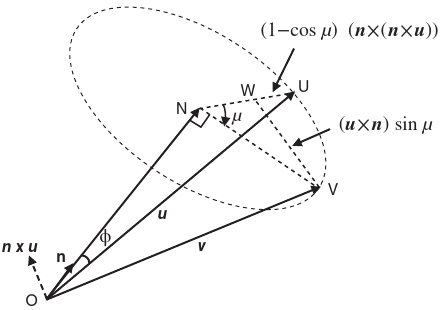
\includegraphics[width=0.5\textwidth, keepaspectratio]{figuras/figure1.2-1.png}\label{fig1.2-1}
    \caption{Rotação de um vetor}\label{fig:rotacao-de-um-vetor}
\end{figure}

Na figura acima, o vetor \(\mathbf{u}\) foi rotacionado para formar o vetor \(\mathbf{v}\) ao definirmos um eixo de rotação ao longo do vetor \(\mathbf{n}\) e realizarmos uma rotação pelo ângulo \(\mu\) ao redor de \(\mathbf{n}\). Estes dois vetores se somam a \(\mathbf{u}\) para obtermos \(\mathbf{v}\), e onde temos que:
    \begin{align*}
     \mathbf{v} &= \mathbf{u} + \left(1 - {\cos{\mu}}\right) \left(\mathbf{n}\!\times\!\left(\mathbf{n}\!\times\!\mathbf{u}\right)\right) - \left(\mathbf{n}\!\times\!\mathbf{u}\right){\sin{\mu}} \tag{1.2-5a}
    \end{align*}
    \begin{align*}
     \mathbf{v} = \left(1 - {\cos{\mu}}\right) \mathbf{n}\!\left(\mathbf{n}\cdot\mathbf{u}\right) + \mathbf{u}{\cos{\mu}} - \left(\mathbf{n}\!\times\!\mathbf{u}\right){\sin{\mu}} \tag{1.2-5b}
    \end{align*}

    As equações acima (1.2-5), às vezes chamadas de \textit{fórmula de rotação}, nos mostram que definindo \(\mathbf{n}\) e \(\mu\) podemos operar sobre \(\mathbf{u}\) com produtos escalares e vetoriais para obter a rotação desejada, independente de sistemas de coordenadas ou magnitude do ângulo.

    Partindo da figura acima, fazemos uma rotação muito pequena \(\delta\mu \ll 1 \text{rad}\), definindo \(\mathbf{v} = \mathbf{u} + \delta \mathbf{u}\), e, aplicando a equação (1.2-5\(a\)) obtemos:
\begin{equation*}
    \delta \mathbf{u} \approx -\!\sin(-\delta\mu)\mathbf{n}\!\times\!\mathbf{u} \approx (\mathbf{n}\!\times\!\mathbf{u})\delta\mu
\end{equation*}

Dividindo por \(\delta t\), no limite onde \(\delta t \rightarrow 0\), definindo \(\mathbf{\omega} \equiv \dot{\mu}\mathbf{n}\), obtemos:

\begin{equation*}
    \dot{\mathbf{u}} = \mathbf{\omega}\!\times\!\mathbf{u}\tag{1.4-1}
\end{equation*}

Esta equação relaciona a velocidade translacional da ponta do vetor \(\mathbf{u}\) ao vetor \(\mathbf{\omega}\). Este vetor \(\mathbf{\omega}\), que denominados \textit{vetor velocidade angular}, constitui-se de um vetor unitário  que define o eixo de rotação, multiplicado pela taxa de rotação. Este é um vetor livre, pode ser trasladado paralelo a si mesmo, e axial, que mudaria de direção caso houvéssemos escolhido uma convenção de sentido horário para a rotação.

Dessa forma podemos associar \(\mathbf{\omega}\) ao sistema de coordenadas fixado no corpo, atribuindo índices que indicam que ele representa a velocidade angular do corpo em relação a outro determinado sistema.

Como vimos, a atitude de um corpo rígido pode ser descrita por uma matriz rotacional variante no tempo, e, pelo teorema de Euler, esse o corpo possui um único \emph{eixo instantâneo de rotação} ao qual o vetor velocidade angular é paralelo, e também único.

\section{Cinemática e Ângulos de Euler}

Um corpo em movimento pode mudar sua atitude, descrita em ângulos de Euler, ao longo do tempo, e neste sentido podemos falar de uma taxa de mudança de cada um desses ângulos de Euler ao longo do tempo. Essas taxas são coisa distintas, é preciso dizer, do vetor velocidade angular do corpo.

Para vincular as taxas de ângulos de Euler, que descrevem a mudança de atitude de um corpo, à sua velocidade angular, procedemos do seguinte modo. Definimos um quadro de referência \(F_{r}\) e um quadro do corpo \(F_{b}\) com vetor velocidade angular relativa \(\omega_{b/r}\) e uma sequencia de ângulos de Euler que define a atitude do corpo, ou seja, a orientação do sistema de coordenadas preso ao corpo em relação ao sistema de referência. Cada taxa de ângulos de Euler informa a direção e magnitude para um determinado vetor velocidade angular sobre um eixo de coordenadas em particular. Esses três vetores somados formam o vetor velocidade angular resultante do veículo cujas taxas de ângulos de Euler estamos tratando. Desse modo podemos encontrar os componentes do vetor velocidade angular resultante.

Em outras palavras, estamos tratando de movimento sobre a Terra, com um sistema de coordenada \(frd\) (\emph{``front'', ``right'', ``down''} - frente, direita, abaixo) preso no corpo, com o sistema \(ned\) (\emph{``north'', ``east'', ``down''} - norte, leste abaixo) no quadro de referência, e uma sequencia ``yaw-pitch-roll'' de ângulos de Euler do sistema \(ned\) para o sistema \(frd\). No caso das equações de Terra plana o sistema \(ned\) é fixado na Terra, e a velocidade angular relativa é aquela do corpo em relação à Terra. No caso mais geral das equações com seis graus de liberdade o sistema \(ned\) se move sobre a Terra, abaixo do corpo, e devemos estabelecer um quadro de referência abstrato que tem sua própria velocidade angular em relação ao sistema da Terra (determinada pela latitude e longitude).

As transformações de coordenadas são:

\begin{align*}
    \mathbf{\omega}^{frd}_{b/r} = \begin{bmatrix} \dot\phi \\ 0 \\0 \end{bmatrix}
    + C_{\phi} \begin{pmatrix}
        \begin{bmatrix} 0 \\ \dot\theta \\ 0 \end{bmatrix}
        + C_{\theta}\begin{bmatrix} 0 \\ 0 \\ \dot\psi \end{bmatrix}
    \end{pmatrix}
\end{align*}

\ldots sendo \(C_{\phi}\) e \(C_{\theta}\)  as rotações (anti-horárias) dos
planos por cada ângulo de Euler em particular, conforme equação (1.3-10). Após
multiplicar as matrizes, teremos:

\begin{align} \tag{1.4-3}
    \mathbf{\omega}^{frd}_{b/r} \equiv \begin{bmatrix} P \\ Q \\ R \end{bmatrix}
    = \begin{bmatrix}
        1 & 0 & -\sin{\theta} \\
        0 & \cos{\phi} & \sin{\phi}\cos{\theta} \\
        0 & -\sin{\phi} & \cos{\phi}\cos{\theta}
    \end{bmatrix}
    \begin{bmatrix}
        \dot\phi \\
        \dot\theta \\
        \dot\psi
    \end{bmatrix}
\end{align}

\ldots sendo \(P\), \(Q\), \(R\), os componentes do vetor velocidade angular do corpo espresso no sistema \(frd\), respectivamente, rolagem (\emph{``roll''}), arfada (\emph{``pitch''}) e guinada (\emph{``yaw''}). A transformação inversa é dada por:

\begin{align} \tag{1.4-4}
    \begin{bmatrix}
        \dot\phi \\
        \dot\theta \\
        \dot\psi
    \end{bmatrix}
    =
    \begin{bmatrix}
        1 & \sin{\phi}\tan{\theta} & \cos{\phi}\tan{\theta} \\
        0 & \cos{\phi} & -\sin{\phi} \\
        0 & \frac{\sin{\phi}}{\cos{\theta}} & \frac{\cos{\phi}}{\cos{\theta}}
    \end{bmatrix}
    \begin{bmatrix}
        P \\ Q \\ R
    \end{bmatrix}
\end{align}

Para simplificar, definimos \(\Phi \equiv \left[\phi \theta \psi \right]^T \) e reescrevemos  (1.4-4) assim:

\begin{equation} \tag{1.4-5}
    \Phi = H \left( \Phi \right) \mathbf{\omega}^{frd}_{b/r}
\end{equation}

As equações (1.4-3) e (1.4-4) serão referidos como as equações cinemáticas de Euler. Note que as matrizes de coeficientes \emph{não são} matrizes ortogonais representando rotações ordinárias de coordenadas. Note ainda que as Equações (1.4-4) e (1.4-4) possuem uma singularidade quando  \(\theta = \pm \frac{\pi}{2}\). Ainda, se essas equações forem utilizadas em uma simulação, as taxas de ângulos de Euler podem integrar para ângulos fora do intervalos de ângulos de Euler, e portanto, seria necessário incluir uma lógica para lidar com essa situação no programa simulador. Não obstante, as equações cinemáticas de Euler são bastante empregadas em simulações.

